% Created 2021-12-12 dom 03:04
% Intended LaTeX compiler: pdflatex
\documentclass{article}
\usepackage[utf8]{inputenc}
\usepackage[T1]{fontenc}
\usepackage{graphicx}
\usepackage{grffile}
\usepackage{longtable}
\usepackage{wrapfig}
\usepackage{rotating}
\usepackage[normalem]{ulem}
\usepackage{amsmath}
\usepackage{textcomp}
\usepackage{amssymb}
\usepackage{capt-of}
\usepackage{hyperref}
\usepackage[spanish]{babel}
\usepackage{pifont}
\usepackage{cancel}
\usepackage{pagecolor,lipsum}
\pagecolor{pink!90!pink}
\setcounter{secnumdepth}{2}
\author{Luis Eduardo Galindo Amaya}
\date{\today}
\title{Cálculo Multivariable}
\hypersetup{
 pdfauthor={Luis Eduardo Galindo Amaya},
 pdftitle={Cálculo Multivariable},
 pdfkeywords={},
 pdfsubject={},
 pdfcreator={Emacs 26.3 (Org mode 9.1.9)}, 
 pdflang={Spanish}}
\begin{document}

\maketitle
\tableofcontents


\section{Preámbulo}
\label{sec:org5866a68}
Este es un trabajo en proceso, todavía no ha sido finalizado y todavía no ha sido revisado. Sí tienes alguna idea para alguna corrección puedes mandarme un correo a mi correo \href{mailto:egalindo54@uabc.edu.mx}{egalindo54@uabc.edu.mx}.

\subsection{Sistema Algebraico Computacional}
\label{sec:org170f070}
Estos apuntes están hechos para usarse en conjunto con el software CAS de George Weigt, Eigenmath, intentare pasar los apuntes a 

\subsection{Especificaciones}
\label{sec:orge2e5ffe}
\begin{itemize}
\item Todos los ángulos son en radianes.
\item Utilizare la notación de subíndices al derivar, por ejemplo \(F_x\) es derivada de la variable 'x' y \(F_{xy}\) es la derivada de 'x' y luego la derivada de 'y'.
\item Cuando escriba un vector usare la notación \vec{A}, prefiero usar las negritas a modo de énfasis.
\item Los diagramas que aparecen aqui son meramente orientativos, por lo tanto pueden ó pueden no representar los nombres de las variables que uso para las explicaciones.
\end{itemize}

\section{Interpretar un plano}
\label{sec:org10cee68}
\subsection{Eje coordenado}
\label{sec:orgc05866f}
Un eje coordenado es una secciona en la que dividimos una región del plano para despumes numerarla, usualmente los llamamos 'x', 'y' y 'z'.

\subsection{Cuadrante}
\label{sec:org015cf38}
En Geometría euclidiana plana recibe el nombre de cuadrante cada una de las cuatro regiones infinitas en que los ejes del Sistema Cartesiano bidimensional dividen al plano. Estos cuadrantes están numerados de 1 al 4 (empezando en el superior derecho, en sentido anti-reloj) y denotados por números Romanos.

\href{https://es.wikipedia.org/wiki/Cuadrante\_(geometr\%C3\%ADa)}{Origen}

\subsection{Octante}
\label{sec:orgdaf75b5}
Un octante en geometría del espacio es cada una de las ocho divisiones coordenadas cartesianas tridimensionales dividen al espacio euclidiano definidos por los signos de las coordenadas. Es similar al cuadrante bidimensional y al semi eje mono-dimensional.

\href{https://es.wikipedia.org/wiki/Octante\_(geometr\%C3\%ADa)}{Origen}

\begin{figure}[htbp]
\centering
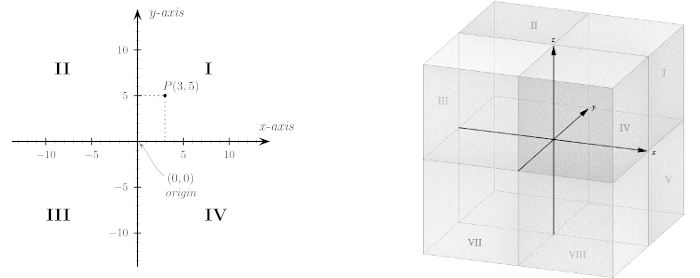
\includegraphics[width=250px]{img/cuadrante-y-octante-2.png}
\caption{A la derecha cuadrantes y a la izquierda los octantes.}
\end{figure}

\section{Representación De Punto En El Plano}
\label{sec:org0748169}
Cuando trabajamos con planos cartesianos podemos marcar puntos indicando el numero de su coordenada en cada respectivo eje, esta una forma muy rápida de interpretar un punto en el espacio, sin embargo no es la única y sobre todo cuando trabajamos con funciones circulares las representaciones rectangulares terminan complicando nuestro trabajo.

\subsection{Rectangular ó Cartesianas}
\label{sec:org3861c72}
Las coordenadas rectangulares, son las coordenadas con las que hemos trabajado todo este tiempo, se representa con un numero en cada eje coordenado y para extenderlo simplemente agregamos un numero extra para cada valor que deseamos representar. 

\begin{figure}[htbp]
\centering
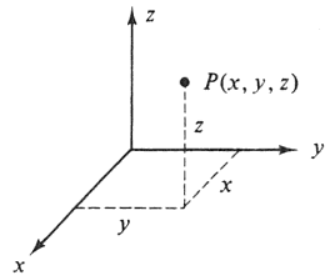
\includegraphics[width=4cm]{img/coordenadas-cartesianas.png}
\caption{Coordenadas Rectangulares.}
\end{figure}

\subsection{Polar ó Cilíndrica}
\label{sec:orga7a5bd3}
Una coordenada polar tiene dos partes principales, una longitud ó radio (r) y un ángulo (\(\theta\)), como cabe imaginar podemos representar figuras circulares con mucha facilidad, también es la notación mas común para vectores en física.

\begin{figure}[htbp]
\centering
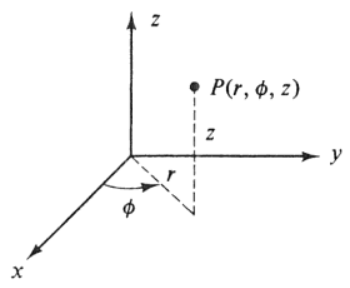
\includegraphics[width=4cm]{img/coordenadas-cilindricas.png}
\caption{Coordenadas Cilíndricas.}
\end{figure}

Podemos extender esta representación en el espacio añadiendo el eje z, el cual nos indicara la altura hacia donde apunta el vector.

\subsection{Esférica}
\label{sec:org7f47dcc}
La representación esférica solo existe en el espacio, y como lo indica su nombre solo representa un valor en el un volumen esférico, esta representación utiliza un radio que abarca los tres ejes (\(\rho\)) dos ángulos para indicar la dirección del punto que deseamos representar, uno para los ejes 'x' y 'y' (\(\theta\)) y uno para el eje 'z' (\(\phi\)).

\begin{figure}[htbp]
\centering
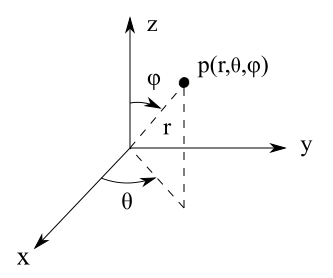
\includegraphics[width=4cm]{img/coordenadas-esfericas.png}
\caption{Coordenadas esféricas.}
\end{figure}

\section{Conversión Entre Sistemas De Coordenadas}
\label{sec:org58d68e9}
Ocasionalmente tenemos que hacer conversiones entre dos ó más sistemas de coordenadas, para hacer estas conversiones es necesario tomar en cuenta las propiedades geométricas de cada sistemas.

\subsection{Rectangulares a Polares}
\label{sec:org6786fb4}
Las Coordenadas polares están compuestas de dos partes, un radio y un ángulo, tenemos dos formulas para calcular cada uno de los componentes: 

\[\begin{aligned}
 r = \sqrt{x^2+y^2} && \theta = arctg\left(y/x\right) \\
\end{aligned}\] 

\textbf{Importante:} Estamos despejando un triangulo y dependiendo el cuadrante donde se encuentre el punto tenemos que sumar los ángulos que nos faltan: 

\begin{center}
\label{tab:orgb677b55}
\begin{tabular}{lll}
Cuadrante & Grados & Radianes\\
\hline
I & 0° & 0\\
II & 180° & \(\pi\)\\
III & 180° & \(\pi\)\\
IV & 360° & 2\(\pi\)\\
\end{tabular}
\end{center}

\subsection{Rectangulares a Cilíndricas}
\label{sec:org3e3c5d9}
las coordenadas cilíndricas son una extencion al espacio de las coordenadas polares por lo tanto solo convertimos las coordenadas de los ejes 'x' y 'y' a polares y añadimos el eje de las 'z' sin hacer ningún cambio.

\href{http://www.learningaboutelectronics.com/Articulos/Calculadora-de-conversion-de-coordenadas-cartesianas-a-cilindricas.php}{Origen}

\subsection{Rectangulares a Esféricas}
\label{sec:org4978744}
Las coordenadas cilíndricas son otra forma de representar las coordenadas polares en el espacio, pero a comparación de las coordenadas cilíndricas ahora usamos dos ángulos para representar la dirección hacia la que apunta el vector: 

\[\begin{aligned}
 \rho = \sqrt{x^2+y^2+z^2} && 
 \theta = arctg\left( y/x \right)  &&
 \phi = arccos\left( z/\rho \right) \\
\end{aligned}\] 

\textbf{Importante I:} el ángulo \(\phi\) (phi) \textbf{NO} necesita corrección.

\textbf{Importante II}: el ángulo \(\theta\) (theta) \textbf{Si} ocupa \hyperref[tab:orgb677b55]{corrección}.

\noindent\rule{\textwidth}{0.5pt}

\subsection{Polares a rectangulares}
\label{sec:orge8a038e}
La conversión de polares a rectangulares se puede hacer directamente con las siguientes formulas: 

\[\begin{aligned}
 x = r \cos(\theta) && y = r \sin(\theta) \\
\end{aligned}\] 

Cada una corresponde a un eje coordenado, recordemos que las coordenadas polares solo sirven para representar puntos en el plano, por lo tanto si queremos representar puntos en el espacio tendremos que usar coordenadas cilíndricas.

\subsection{Polares a cilíndricas}
\label{sec:orgc1eda9b}
Las coordenadas cilíndricas son la extencion directa de las coordenadas polares en el espacio, por lo tanto simplemente tendremos que tomar el valor rectangular de nuestra coordenada en el eje 'z' y añadirla a nuestra representación polar.

\subsection{Cilindricas a Rectangulares}
\label{sec:org4ff2f1f}
Para esta conversión simplemente tenemos que hacer las siguientes sustituciones:

\[\begin{aligned}
 x = r \cos(\theta) && y = r \sin(\theta) && z = z \\
\end{aligned}\] 

\href{https://www.neurochispas.com/wiki/coordenadas-cilindricas-a-cartesianas/}{Origen}

\subsection{Cilíndricas a Esféricas}
\label{sec:org7e44b6d}
Para hacer esta conversión es necesario extender el radio a tres dimensiones y calcular el ángulo faltante, como ya tenemos el ángulo \(\theta\) (theta) no tenemos que hacer correcciones.

\[\begin{aligned}
 \rho = \sqrt{r^2+z^2} && 
 \theta = \theta  &&
 \phi = arccos\left( z/\rho \right) \\
\end{aligned}\] 

\href{http://www.learningaboutelectronics.com/Articulos/Calculadora-de-conversion-de-coordenadas-cilindricas-a-esfericas.php}{Origen - 1} | \href{https://math.libretexts.org/Bookshelves/Calculus/Book:\_Calculus\_(OpenStax)/12:\_Vectors\_in\_Space/12.7:\_Cylindrical\_and\_Spherical\_Coordinates\#:\~:text=To\%20convert\%20a\%20point\%20from,r2+z2).}{Origen - 2}

\noindent\rule{\textwidth}{0.5pt}

\subsection{Esféricas a Rectangulares}
\label{sec:org5890657}
Para esta conversión simplemente tenemos que hacer las siguientes sustituciones:

\[\begin{aligned}
 x = \rho \sin(\phi)\cos(\theta) && 
 y = \rho \sin(\phi)\sin(\theta) &&
 z = \rho \cos(\phi) \\
\end{aligned}\] 

\href{https://www.neurochispas.com/wiki/coordenadas-esfericas-a-cartesianas/}{Origen}

\subsection{Esféricas a Cilíndricas}
\label{sec:orgeebbb9f}
para convertir las coordenadas esféricas a cilíndricas tendremos que convertir el ángulo \(\phi\) (phi) a su coordenada cartesiana 'z':

\[\begin{aligned}
 r = \rho \sin(\phi) && 
 \theta = \theta &&
 z = \rho \cos(\phi) \\
\end{aligned}\] 

\href{https://temasdecalculo.com/2017/12/18/4-14-coordenadas-cilindricas-y-coordenadas-esfericas-calculo-vectorial/}{Origen}

\noindent\rule{\textwidth}{0.5pt}

\section{Vectores}
\label{sec:org7ba5718}
Un vector es la representación matemática y gráfica de una magnitud vectorial. Consiste básicamente en una flecha o segmento rectilíneo orientado, es decir, con una determinada longitud, dirección y sentido, y que contiene toda la información de la magnitud que se está midiendo. Ejemplos de vectores: 

\[\begin{aligned}
  (x,y,z) && (r,\theta) && (\rho, \theta, \phi) \\
\end{aligned}\] 

\href{https://ingemecanica.com/tutoriales/calculo\_vectorial.html}{Origen}

\subsection{Representación}
\label{sec:orgadf1af5}
En física usualmente se representan los vectores de forma polar ó cilíndrica, con una magnitud y un ángulo, pero esto no tiene por que ser siempre así, en calculo multivariable con mucha frecuencia se utiliza la la notación cartesiana (tres números dentro de un paréntesis representando cada eje coordenado) ó también la compleja (donde cada uno componentes es una variable 'i' es x 'j' es 'y' y 'z' es 'k'), ejemplo el vector (1,3,4) se puede representar de manera compleja como el punto 'i + 3j + 4k'. 

\subsection{Notación}
\label{sec:org38d4339}
Para identificar que un valor es un vector hay dos formas principales añadiendo una flecha en la parte superior de la variable (\(\vec{A}\)) o resaltando el nombre de la variable con negritas. 

\subsection{Vector Negativo}
\label{sec:org36a0a59}
Si un vector tiene el simbolo negativo, todos sus componentes cambian su signo: 

\[
-\vec{A} = (-\vec{A_1},-\vec{A_2},...,-\vec{A_n})
\]

\uline{Esto si el vector esta en coordenadas rectangulares}, cuando el vector esta en polar añadimos 180° grados al ángulo: 

\[ \begin{aligned}
\vec{A} = (3,75^\circ) && -\vec{A} = (3,-75^\circ) = (3,255^\circ)
\end{aligned} \]

\subsection{Suma y Resta de Vectores}
\label{sec:orga525f19}
Sumar vectores no representa mas que la suma de independiente de cada uno de sus componentes.

\[
\vec{A} + \vec{B} = (\vec{A}_x + \vec{B}_x,\vec{A}_y + \vec{B}_y,\vec{A}_z + \vec{B}_z)
\]

\[
\vec{A} - \vec{B} = (\vec{A}_x - \vec{B}_x,\vec{A}_y - \vec{B}_y,\vec{A}_z - \vec{B}_z)
\]

\textbf{Importante:} Esto es solo para coordenadas cartesianas, si tenermos nuestro vector en coordenadas cilíndricas ó esféricas tendremos que hacer la conversión correspondiente.

\subsection{Multiplicación Escalar}
\label{sec:org86eb149}
Podemos multiplicar un vector por un valor fijo para aumentar su tamaño, simplemente multiplicamos cada componente por la constante de nuestro interés:

\[
k \cdot \vec{A} = (k\cdot\vec{A_x},k\cdot\vec{A_y},k\cdot\vec{A_z})
\]

\subsection{Modulo ó magnitud del Vector}
\label{sec:org79110b0}
El módulo de un vector es la longitud entre el inicio y el final del vector, podemos calcular la distancia desde el origen con la formula de distancia:

\[
\vert\vec{A}\vert = \sqrt{ x^2 + y^2 + z^2 }
\]

\subsubsection*{Modulo del Vector Fuera Del Origen}
\label{sec:org91db1a4}
Hay ocaciones en las que tenemos un vector que no parte desde el origen de nuestra gráfica, para eso simplemente tenemos que restar al vector el punto de origen, por ejemplo sí tenemos un vector \(\vec{A} = (3,5,6)\) con origen en \(g = (5,6,3)\) simplemente las restamos:

\[ \begin{aligned}
\vec{A} &= (3-5,5-6,6-3) \\
~ &= (-2,-1,3) \\
\end{aligned} \]

De este modo podemos calcular la magnitud del vector independientemente de su origen:

\[ \begin{aligned}
\vec{A} &= (-2,-1,3) \\
\vert\vec{A}\vert &= \sqrt{14} \\
\end{aligned} \]

\subsection{Producto Punto}
\label{sec:org0f3c51d}
Para representar el producto punto usamos el operador \(\cdot\). Al producto punto también se le llama comúnmente producto escalar ya que el resultado \uline{siempre es una escalar}. Es producto punto en palabras sencillas es la suma de la multiplicación de componente por componente:

\[\vec{A} \cdot \vec{B} = \vec{A}\vec{B}^T\].

\[
\vec{A} \cdot \vec{B} = \vec{A}_1 \vec{B}_1 + \vec{A}_2 \vec{B}_2 + ... + \vec{A}_n \vec{B}_n
\]

Una propiedad muy importante que debemos tener en cuenta es su relacion con los ángulos de los vectores, esto es muy útil para determinar los ángulos directores más adelante:

\[
 \vec{A}\cdot\vec{B} = \vert\vec{A}\vert\vert\vec{B}\vert \cos(\theta)
\]

\subsection{Producto Cruz}
\label{sec:orgd4ec638}
El producto cruz al igual que el producto punto representa una operacion que raciona dos vectores y sus maginitudes, su operador es \(\times\), a comparacion del producto punto el resultado \uline{No es un escalar}, el producto cruz siempre devuelve otro vector:

\[
\vec{A} \times \vec{B} = \det\begin{pmatrix}
       i    &      j    &     k    \\
  \vec{A_x} & \vec{A_y} & \vec{A_z}\\
  \vec{B_x} & \vec{B_y} & \vec{B_z}\\
\end{pmatrix}
\]

\[
\vec{A} \times \vec{B} = 
  (\vec{A_y}\vec{B_z} - \vec{A_z}\vec{A_y})i + 
  (\vec{A_z}\vec{B_x} - \vec{A_x}\vec{A_z})j + 
  (\vec{A_x}\vec{B_y} - \vec{A_y}\vec{A_x})k
\]

Al igual que el producto punto el producto cruz representa la relación geométrica, la formula es muy parecida mas sin embargo ahora usamos el seno en vez del coseno, entre dos vectores:

\[
\vert \vec{A}\times\vec{B}\vert = \vert\vec{A}\vert\vert\vec{B}\vert \sin(\theta)
\]

\section{Aplicaciones De Vectores}
\label{sec:org2ef1586}
\subsection{Vector Unitario}
\label{sec:org2887bbe}
La característica fundamental del vector unitario es que su longitud siempre es igual a '1', no importa la dirección o el cuadrante mientras el modulo es igual a '1' entonces es unitario. El vector unitario es muy util para determinar la direccion de un vector sin tener que tomar en cuenta su magnitud. Para calcularlo simplemente dividimos los valores de nuestro vector entre el modulo.

\[ 
\hat{A} = \frac{\vec{A}}{\vert\vec{A}\vert} 
\]

\subsection{Ángulos Entre Vectores}
\label{sec:orga61789d}
Si recordamos una de las propiedades de el producto punto y el producto cruz es que representan la relación entre el ángulo y las magnitudes de los vectores:

\[ \begin{aligned}
 \vec{A}\cdot\vec{B} = |\vec{A}||\vec{B}| \cos(\theta) && |\vec{A}\times\vec{B}| = |\vec{A}||\vec{B}| \sin(\theta) \\
\end{aligned} \]

Entonces si despejamos los vectores obtenemos las siguientes formulas:

\[ \begin{aligned}
\cos(\theta) = \frac{\vec{A} \cdot \vec{B}}{|\vec{A}||\vec{B}|} &&
\sin(\theta) = \frac{|\vec{A}\times\vec{B}|}{|\vec{A}||\vec{B}|} \\
\end{aligned} \]

\subsection{Ángulos Directores}
\label{sec:orgccc6be4}
Es aquel entre un vector y uno de los ejes (ya sea 'x', 'y' ó 'z'), para calcularlo solo tenemos que medir el ángulo entre nuestro vector y el eje que nos interesa conocer:

\[\begin{aligned}
  \cos(\alpha) = \frac{a_x}{|\vec{a}|} &&
  \cos(\beta)  = \frac{a_y}{|\vec{a}|} &&
  \cos(\gamma) = \frac{a_z}{|\vec{a}|} \\
\end{aligned} \]

\begin{figure}[htbp]
\centering
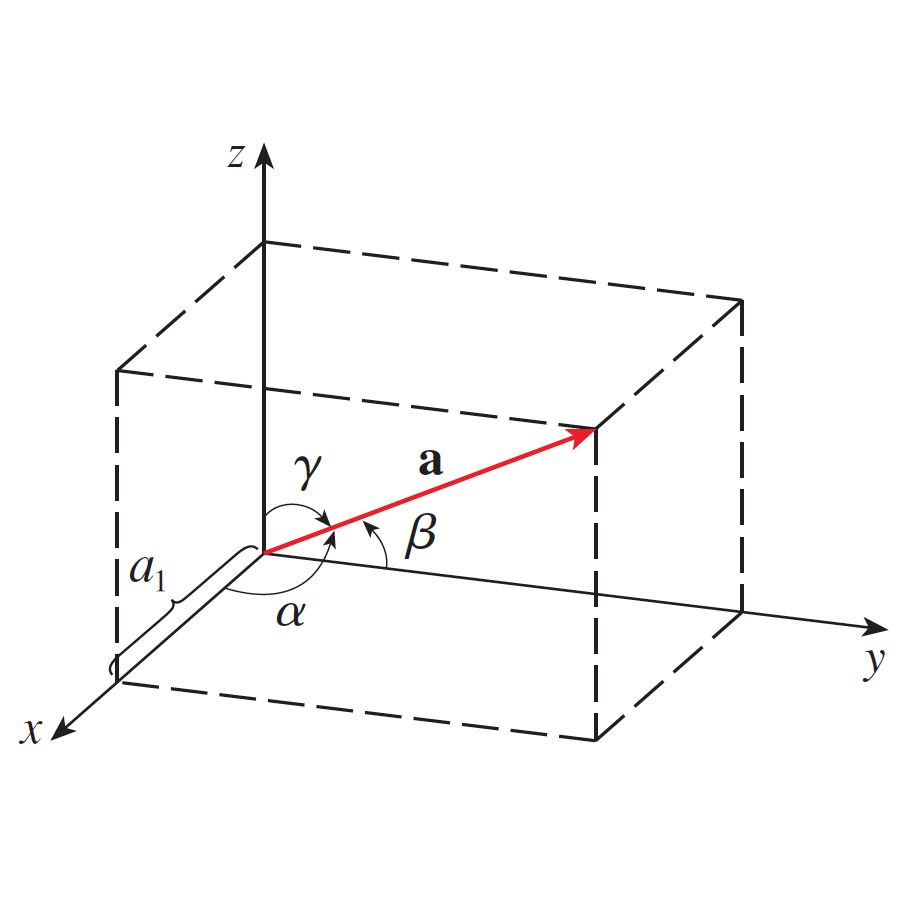
\includegraphics[width=4cm]{img/angulos-directores.png}
\caption{Ángulos directores de \(\vec{a}\).}
\end{figure}

\href{https://www.superprof.es/diccionario/matematicas/analitica/cosenos-directores.html}{Origen}

\subsubsection*{Despeje Del Los Ángulos Directores:}
\label{sec:org9c02d42}
Estas formulas se despejan de la formula del producto punto, como es un vector unitario sobre cada eje los valorse que no usamos se anulan automáticamente\footnote{También es posible usar el producto cruz para este procedimiento, pero por simplicidad se prefiere el producto punto.}:

\[\begin{aligned}
  cos(\alpha) &= \frac{a_x \cdot 1 + \cancel{a_y \cdot 0~} + \cancel{a_z \cdot 0} }{|\vec{a}| \cdot \sqrt{1^2+\cancel{0^2}+\cancel{0^2}}} \\
  cos(\alpha) &= \frac{a_x \cdot 1}{|\vec{a}| \cdot 1} \\
  cos(\alpha) &= \frac{a_x}{|\vec{a}|} \\
\end{aligned} \]

\subsection{Área De Un Paralelogramo}
\label{sec:orgcc81bc2}
Si tenemos dos vectores podemos calcular el area del del paralelogramo que se forma simplemente usando el producto cruz, Esto lo podemos verificar son el siguiente diagrama:

\begin{figure}[htbp]
\centering
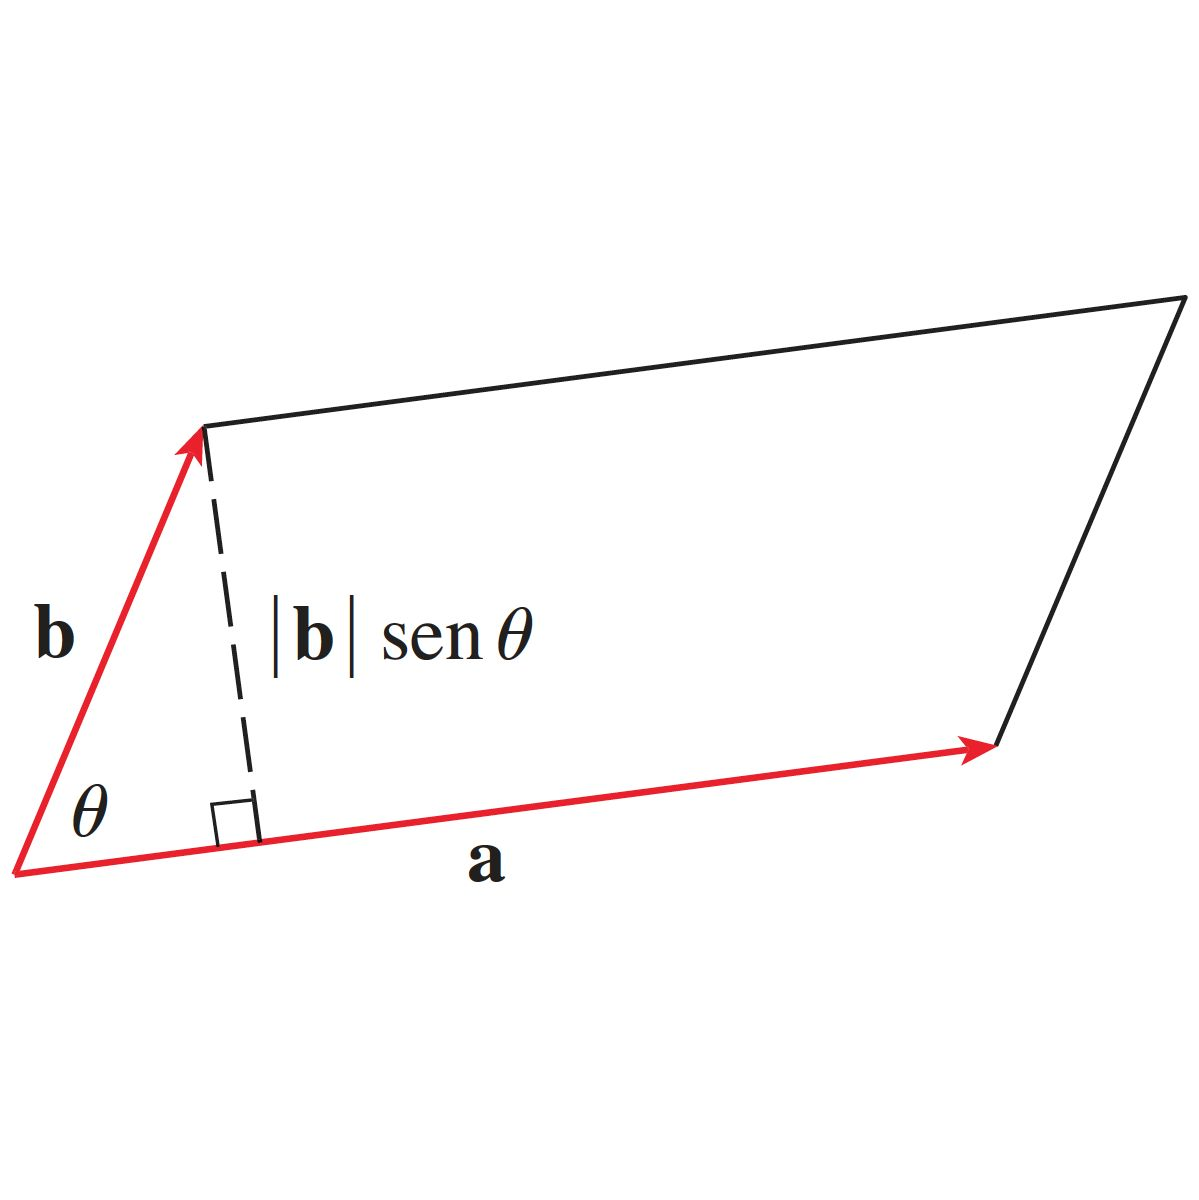
\includegraphics[width=4cm]{img/producto-cruz.png}
\caption{El paralelogramo se parece al rectangulo pero inclinado.}
\end{figure}

En primaria aprendimos que el área del paralelogramo es base por altura, sin embargo la altura del paralelogramo no se puede obtener midiendo sus lados ya que esta inclinado, si aplicamos trigonometría podemos saber que el valor del cateto opuesto (la altura) es igual al seno del angulo, entonces la formula quedaria:

\[
\text{Área} = \text{base} \cdot \sin(\theta)
\]

Y esto es exactamente a el valor de el producto cruz de dos vectores:

\[
{|a||b|\sin(\theta) = |a \times b|}
\]

\subsection{Volumen De Un Paralelepípedo}
\label{sec:orgd971413}
\end{document}
